
	La información del presente documento se encuentra estructurada mediante diagramas, tablas y secciones con nomenclaturas y estándares específicos. También se utiliza un código de colores para representar ciertos elementos no soportados por el lenguaje. Este capítulo tiene como finalidad indicar la forma en que se deben leer estos elementos para un mejor entendimiento.
%---------------------------------------------------------
\section{Modelado del negocio}

	Para modelar el negocio, se presenta el glosario de términos, el modelado de la estructura de la información que tendrá el sistema, las reglas de negocio que rigen las operaciones y máquinas de estados para modelar los ciclos de gestión en el CALMÉCAC. En esta sección describimos las notaciones y códigos de colores usadas en dichas secciones.

%- - - - - - - - - - - - - - - - - - - - - - - - - - - - -
\subsection{Modelado de estructura de datos}
\label{sec:ModeladoDatos}

	Esta sección presenta el modelo de la información (entidades, atributos y referencias) que manejará el CALMÉCAC con base en el negocio. Para esto se construye un diagrama de clases en el que se especifican:

\begin{itemize}
	\item Entidades: como Clases.
	\item Atributos: Especificando el nombre y el tipo de dato.
	\item Relaciones: Especificando el rol que juega una entidad con otra, el tipo de relación (de agregación, composición o generalización) y la cardinalidad.
\end{itemize}

Todo esto se modela utilizando \href{http://www.omg.org/spec/UML/2.0/}{UML 2.0}.\\


Para describir  cada uno de los atributos de una entidad se utiliza una tabla que contiene las siguientes columnas:

\begin{description}
	\item[Nombre:] Indica el nombre del atributo.
	\item[Tipo:] Indica que tipo de dato es el atributo.
	\item[Descripción:] Ayuda a entender a que se refiere el atributo.
	\item[Req:]  Indica si un atributo es obligatorio (requerido) u opcional.
\end{description}

	Las relaciones del diagrama de clases se describen por cada entidad relacionada en una tabla con las siguientes columnas:

\begin{description}
	\item[Tipo:] Específica el tipo de relación que puede ser:
		\begin{itemize}
			\item \textbf{Agregación}: Es aquella relación que indica que una entidad es utilizada o se conforma de entidades más pequeñas pero puede existir por si sola y se denota por el símbolo \brRelAgregation.
			\item \textbf{Composición} : Es aquella relación que indica que una entidad necesita de otra para poder existir y si alguna de las dos se borra la otra también será eliminada. Se denota por el símbolo \brRelComposition.
			\item \textbf{Generalización}: Es aquella relación que indica que una entidad \textit{hereda} de otra y se denota por el símbolo \brRelGeneralization.
		\end{itemize}
	\item[Descripción:] Proporciona una redacción de un enunciado que ayuda a comprender el porque de la relación.
	\item[Rol:] Indica el rol que tiene la entidad de acuerdo al tipo de relación.
\end{description}

%- - - - - - - - - - - - - - - - - - - - - - - - - - - - -
%\subsection{Código de colores para diagramas de clases}

%	Para las clases  que representan catálogos o tipos primitivos, se usará un relleno (\textit{fill}) \textit{Gray} al 80\% transparencia como se muestra en la figura \ref{fig:Catalogo}

%\begin{figure}[hbtp!]
%	\begin{center}
%		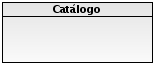
\includegraphics[width=.25\textwidth]{introduccion/images/Catalogos}
%	\end{center}
%	\label{fig:Catalogo}
%	\caption{Clase Catálogo}
%\end{figure}

%Para las demás clases actualmente se puede usar cualquier color.
%- - - - - - - - - - - - - - - - - - - - - - - - - - - - -
\subsection{Modelado de reglas de negocio}

Las reglas de negocio son directivas que tienen como fundamento la misión de un negocio y como objetivo gobernar estrategias y tácticas para poder conseguir esta misión. Una regla de negocio es practicable ya que no requiere de una interpretación adicional. Estas reglas también son una fuente de información muy relevante ya que generalmente establecen las relaciones entre dos o más términos del negocio.

En el documento se presentarán estas reglas en forma de secciones indicando los siguientes atributos:

\begin{description}
	\item[Id:] Es el identificador de la regla de negocio con la cual se podrá referenciar a lo largo del documento.
	\item[Nombre:] Indica el nombre de la regla de negocio el cual debe describir de forma concisa en que consiste la regla.
	\item[Tipo:] Indica el tipo de regla de negocio de acuerdo a como se aplica.
		\begin{itemize}
			\item Habilitadora: Permite realizar el proceso en el que la regla se ve involucrada.
			\item Cronometrada: Recibe parámetros y con respecto a eso realiza el proceso.
			\item Ejecutiva: Es aquella que se debe llevar a cabo cuando una autoridad se ve involucrada para que el proceso concluya.
		\end{itemize}
	\item[Clase:] Indica la naturaleza de la regla de negocio.
		\begin{itemize}
			\item Condición: Es una regla que cumple una condición para llevarse a cabo.
			\item Integridad Referencial: Es una regla que indica validaciones que, de no ser tomadas en cuenta se pondría en peligro la integridad de la información.
			\item Autorización: Son restricciones en las que se ven involucradas palabras como, al menos uno.
		\end{itemize}

	\item[Nivel:] Indica como es que la regla se toma en cuenta para el desarrollo del Calécac.
		\begin{itemize}
			\item Controla: Define que el sistema se encargará de vigilar el cumplimiento de la regla en todo momento.
			\item Influencia: Sugiere formas en las que debería realizarse la operación, pero no la limita. De tal forma que el sistema dará facilidades para evitar esas situaciones o advertirá cada vez que se detecte que la regla no es tomada en cuenta.
		\end{itemize}

	\item[Descripción:] Es un pequeño resumen que ayuda a entender la regla de negocio.
	\item[Motivación:] La razón detrás de la existencia de la regla de negocio.
	\item[Sentencia:] Descripción formal o matemática de la regla de negocio.
	\item[Ejemplo Positivo:] Describe ejemplos en los que la regla se cumple.
	\item[Ejemplo Negativo:] Describe ejemplos en los que la regla no se cumple.
\end{description}

%- - - - - - - - - - - - - - - - - - - - - - - - - - - - -
\section{Modelado de casos de uso}

	Los diagramas de casos de uso son una herramienta usada para representar las transacciones entre un actor y el sistema, las cuales siempre tendrán un valor agregado o un propósito para que el actor las realice.
En estos diagramas se podrán observar los siguientes elementos:

\begin{itemize}
	 \UCpaso Representa al sistema. Es un óvalo y el cómo haga las acciones definidas en las trayectoria es algo que no compete a este documento.
	\item \UCactor Representa al actor.
	\item Relación $<$- - -$<<extends>>$- - -. Indica que un caso de uso \textbf{puede} ejecutarse a partir de otro.
	\item Relación - - -$<<include>>$- - -$>$. Indica que un caso de uso \textbf{debe} ejecutarse a partir de otro.
\end{itemize}

La conexión entre un actor y un caso de uso es por medio de una línea como se muestra en la figura \ref{fig:acUC}.

\begin{figure}[hbtp!]
	\begin{center}
		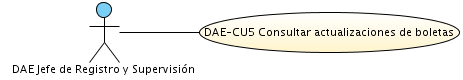
\includegraphics[width=.4\textwidth]{introduccion/images/ActorUC}
	\end{center}
	\label{fig:acUC}
	\caption{Un Actor y un caso de uso}
\end{figure}

Los casos de uso se encontrarán dentro de paquetes (representados por carpetas) indicando así que pertenecen a un mismo módulo del Calmécac como se muestra en la figura \ref{fig:pack}.

\begin{figure}[hbtp!]
	\begin{center}
		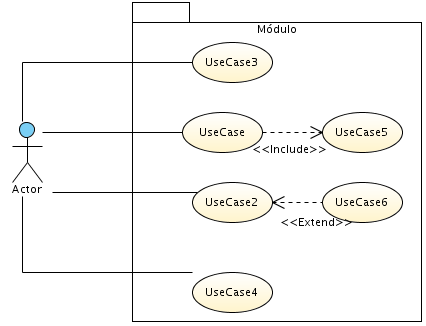
\includegraphics[width=.4\textwidth]{introduccion/images/Paquete}
	\end{center}
	\label{fig:pack}
	\caption{Un Actor con varios caso de uso dentro de un módulo}
\end{figure}

\pagebreak

%- - - - - - - - - - - - - - - - - - - - - - - - - - - - -
%\subsection{Código de colores para diagramas de casos de uso}

%Los casos de uso tendrán un color \textit{Gradient Golden} con 80\% de transparencia; los actores tendrán un  \textit{fill} \textit{RGB(122,207,245)}; los módulos del Calmécac tendrán un relleno (\textit{fill}) de color \textit{White} al 70\% de transparencia y por último el Calmécac se representa con un rectángulo de \textit{fill} \textit{RGB(128,0,0)} al 80\% de transparencia.

%- - - - - - - - - - - - - - - - - - - - - - - - - - - - -
\subsection{Identificadores de casos de uso}

Los casos de uso se identificarán de acuerdo a la siguiente nomenclatura:

\begin{figure}[hbtp!]
	\begin{center}
		
\includegraphics[width=.7\textwidth]{introduccion/images/UCnombre}
	\end{center}
	\label{fig:nomenclatura}
	%\caption{Nomenclatura de un caso de uso}
\end{figure}



En donde los subsistemas son:
\\
\begin{Titemize}
	\Titem [HR:] Horarios
	\Titem [SD:] Soporte Documental
\end{Titemize}

En donde división puede ser únicamente el módulo o el módulo puede tener submódulos.\\
 En el subsistema Horarios existe la división de módulos:\\
\begin{Titemize}
	\Titem [UA:] Unidad Académica
	\Titem [PR:] Profesor
	\Titem [EE:] Estructura Educativa
\end{Titemize}
\cdtEmpty
\\En el módulo Unidad académica se divide en submódulos:\\
\begin{Titemize}
	\Titem [GG:] Gestionar Grupo
	\Titem [CO:] Consultas
\end{Titemize}

En el subsistema Soporte Documental existe la división de módulo:\\
\begin{Titemize}
	\Titem [AP:] Aprobación
\end{Titemize}


\textbf{Ejemplo positivo} Cumple con la nomenclatura:
\begin{itemize}
	\item HR-UA-CU4 Gestionar oferta educativa
	\item HR-UA-GG-CU1.3 Asignar profesor
	\item SD-UA-CU1 Gestionar soporte documental por formatos
\end{itemize}


\textbf{Ejemplo negativo} No cumple con la nomenclatura:
\begin{itemize}
	\item CU7-UA-HR Gestionar oferta educativa
	\item GG-CU-UA3.1 Asignar profesor
\end{itemize}


%- - - - - - - - - - - - - - - - - - - - - - - - - - - - -
\subsection{Atributos de casos de uso}

Para poder entender un caso de uso más allá de un diagrama se utilizan secciones en el documento para cada uno, dividido por capítulos de acuerdo al subsistema y una tabla con los siguientes datos:

\begin{description}
	\item[Id] Identificador.
	\item[Nombre] Nombre del caso de uso el cual es descriptivo basándose en la tarea que se realiza.
	\item[Actores] Lista de los actores relacionados o que utilizan el caso de uso.
	\item[Descripción] Es un resumen en el que se especifica la transacción.
	\item[Propósito] Indica el objetivo por el cual el caso de uso existe.
	%\item[Operación:] Indica el tipo de operación que realiza el caso de uso.
	\item[Entradas] Lista los datos de entrada que el caso de uso recibe.
	\item[Salidas] Lista los datos de salida que el caso de uso genera.
	\item[Origen] Indica de donde provienen los datos de entrada.
	\item[Destino] Indica a donde se dirigen los datos de salida.
	\item[Precondiciones] Enlista las cosas que deben haber sucedido para que el caso  de uso se lleve a cabo.
	\item[Postcondiciones] Enlista las cosas que suceden en el sistema o negocio de forma inmediata o a corto plazo.
	\item[Errores] Enlista las situaciones en las que el caso de uso concluye sin éxito.
	\item[Reglas de Negocio] Lista las reglas de negocio que están asociadas al caso de uso.
%	\item[Proceso:] Enlista aquellos procesos a los que el caso de uso esta asociado.
%	\item[Subproceso:] Enlista aquellos Subprocesos en los que el caso de uso se aplica.
	\item[Disparadores] Aquellas condiciones o motivaciones que el actor tiene para ejecutar el caso de uso.
	\item[Condición de Término] Aquellos resultados que garantizan que el caso de uso se ha ejecutado con éxito.
	\item[Efectos Colaterales] Afectaciones en otras partes del sistema.
	\item[Viene de] Indica cuando el caso de uso se extiende de otro o se incluye en otro.
\end{description}

%---------------------------------------------------------
\section{Modelado de interfaces}

Una interfaz de usuario permite mostrar la interacción entre un actor y todas las funcionalidades que el sistema ofrece y que le corresponden de acuerdo a su perfil. Para poder modelar estos elementos se describe:
\begin{itemize}
	\item Objetivo: Indica el propósito de las interfaces de usuario (pantallas) y como ayudará al actor a realizar sus tareas.
	\item Descripción: En este apartado se indica y especifica que acciones el actor puede realizar así como la especificación de algunos comportamientos dinámicos en las pantallas.
\end{itemize}

%\subsection{Atributos de las interfaces}
%
%	Los diferentes atributos que se encuentran definidos a partir del capítulo \ref{part:Interaccion} de este documento. Muchos de estos elementos aun no quedan definidos, pero se utilizan símbolos con los cuales el actor pueda identificar o visualizar las acciones y funcionalidades que se pueden realizar oprimiendo estos íconos.

%---------------------------------------------------------
\section{Modelado de mensajes}

Los mensajes son elementos en el sistema que ayudan a mantener pendiente al actor, ya sea para indicarle que la operación se llevó a cabo correctamente, así como alertar de una operación que requiere realizar para poder continuar con procesos específicos realizados en el Instituto.

\subsection{Atributos de mensajes}
Un mensaje se conformará de :
\begin{description}
	\item[Tipo] Indica a que clase pertenece un mensaje, entre las cuales se encuentran:
		\begin{itemize}
			\item \textbf{Informativo:} Notificar al actor que una operación concluyó o para notificar al actor de una operación realizada en el sistema.
			\item \textbf{Confirmación:} Requiere la confirmación del actor para llevar a cabo una operación en el sistema.
			\item \textbf{Error:} Notificar al actor que la operación no se llevo a cabo adecuadamente o no se llevó a cabo.
			\item \textbf{Alerta:} Notificar al actor que una operación requiere de su atención para llevarse a cabo.
		\end{itemize}
	\item[Canal] Indica el medio que el sistema utiliza para enviar un mensaje.
	\item[Propósito] Indica la razón por la cual el mensaje es necesario.
	\item[Redacción] Indica el texto que el actor podrá visualizar cuando el mensaje se muestre.
	\item[Parámetros] Indica un elemento dentro del texto del mensaje que puede cambiar dinámicamente de acuerdo a la operación que se este llevando a cabo.
	\item[Ejemplo] Muestra una aplicación del mensaje.
	\item[Referenciado por] Indica la lista de casos de uso que utilizan el mensaje.
\end{description}

\subsection{Identificadores de mensajes}
Para poder identificar un mensaje, este se compondrá de:
\begin{description}
	\item [Identificador] Indica el número asignado para el mensaje.
	\item [Nombre] Es un resumen de lo que el mensaje realiza/muestra.
\end{description}
